\documentclass[twoside,10pt]{report}
\usepackage{/Users/bradenhoagland/latex/styles/toggles}
\toggletrue{sectionbreaks}
%\toggletrue{sectionheaders}
\newcommand{\docTitle}{Real Analysis}
\usepackage{/Users/bradenhoagland/latex/styles/common}
\usepackage{/Users/bradenhoagland/latex/styles/colors}

%\renewcommand{\theenumi}{\alph{enumi}}

\begin{document}
\tableofcontents


%===================
%===================
% Euclidean Topology
%===================
%===================

\chapter{Euclidean Topology}

%%%%%%%%%%%%%%%%%%%%
% Metrics
%%%%%%%%%%%%%%%%%%%%

\section{Metrics}

\begin{defn}[]
	A \textbf{metric space} $(M,d)$ is a set $M$ and a function $d: M \times M \to \mathbb{R}$ such that
	\begin{enumerate}
		\item $d(x,y) \geq 0$ 
		\item $d(x,y) = 0 \iff x=y$ 
		\item $d(x,y) = d(y,x)$ 
		\item $d(x,y) \leq d(x,z) + d(z,y)$
	\end{enumerate}
\end{defn}

\begin{ex}[]
	 The \textbf{discrete metric} is defined $d(x,y)=1$ if $x\neq y$, $d(x,y)=0$ if $x=y$. For any set $S$, $(S,d)$ is a metric space.
\end{ex}

%%%%%%%%%%%%%%%%%%%%
% Open Sets
%%%%%%%%%%%%%%%%%%%%

\section{Open Sets}

\begin{defn}[]
	Let $(M,d)$ be a metric space. For each fixed $x\in M$ and $\varepsilon>0$, the \textbf{$\varepsilon$-ball} about $x$ is
	\[
		D(x,\varepsilon) = \left\{ y \in M \;|\; d(x,y) < \varepsilon \right\}.
	\] 
\end{defn}

\begin{defn}[]
	A set $A  \subset M$ is \textbf{open} if for every $x \in A$, there exists an $\varepsilon>0$ such that $D(x,\varepsilon) \subset A$. A \textbf{neighborhood} of $x$ in $M$ is an open set containing $x$.
\end{defn}

\begin{figure}[H]
	\centering
	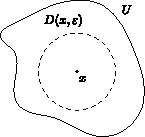
\includegraphics[scale=2]{fig/neighborhood.pdf}
	\caption{A neighborhood $U$ of $x$.}
\end{figure}

\begin{prop}
	In a metric space, every $\varepsilon$-ball $D(x,\varepsilon)$ is open for $\varepsilon>0$.
\end{prop}

\begin{prop}
	In $(M,d)$ with open sets $U_i$,
	\begin{enumerate}
		\item $\bigcap_{i=1}^N U_i$ is open
		\item $\bigcup_{\alpha \in A} U_\alpha$ is open
		\item $\varnothing$ and $M$ are open
	\end{enumerate}
\end{prop}

\begin{ex}[]
	Let $U_n = \left( -\frac{1}{n}, \frac{1}{n} \right)$, then $\bigcap_{n=1}^\infty U_n = \left\{ 0 \right\}$, which is not open. Thus statement (1) does not hold for arbitrary collections of open sets.
\end{ex}

\begin{defn}[]
	The \textbf{interior} of $A \subset (M,d)$ is the union of all open subsets of $A$.
\end{defn}

A point $a \in A$ is an \textbf{interior point} of $A$ if there's a neighborhood of $a$ contained in $A$. Then $A^{o}$ is all the interior points of $A$.

Since $A^o$ is open, $A^o$ is the largest open subset of $A$. Thus if $A$ has no open subsets, then $A^o=\varnothing$. Furthermore, if $A$ is open, then $A^o=A$.


%%%%%%%%%%%%%%%%%%%%
% Closed Sets
%%%%%%%%%%%%%%%%%%%%

\section{Closed Sets}
\begin{defn}[]
	A set $B$ in a metric space $M$ is said to be \textbf{closed} if its complement $B^c = M\backslash B$ is open.
\end{defn}
It's possible for a set to be neither open nor closed (consider $(0,1] \in \mathbb{R}$).

\begin{prop}
        In $(M,d)$ with open sets $C_i$,
        \begin{enumerate}
                \item $\bigcup_{i=1}^N U_\alpha$ is closed
                \item $\bigcap_{\alpha\in A} C_\alpha$ is closed
                \item $\varnothing$ and $M$ are closed
        \end{enumerate}
\end{prop}
\begin{proof}
	These follow from DeMorgan's Laws and the corresponding properties of open sets.
\end{proof}

\begin{ex}[]
Any finite set in $\mathbb{R}^n$ is closed since it is the union of finitely many single points, which themselves are closed sets.
\end{ex}

\begin{ex}[]
	Let \[F_n = \left[\frac{1}{n}, 1-\frac{1}{n}\right] .\] The union $\bigcup_{j=1}^\infty F_j = (0,1)$, so the union of an arbitrary collection of closed sets is not necessarily closed.
\end{ex}

%%%%%%%%%%%%%%%%%%%%
% Accumulation Points
%%%%%%%%%%%%%%%%%%%%

\section{Accumulation Points}
\begin{defn}[]
	A point $x \in M$ is an \textbf{accumulation point} of $A \subset M$ if neighborhood $U$ of $x$ intersects $A$ at a point other than $x$. The set of accumulation points of $A$ is denoted by $\text{acc}(A)$.
\end{defn}

Other points of $A$ get arbitrarily close to $x$ if $x$ is an accumulation point. This means there are infinitely many points of $A$ that are close to $x$.

An accumulation point of a set doesn't need to be in the set itself. A set also doesn't need to have any accumulation points in the first place.

\begin{figure}[H]
	\centering
	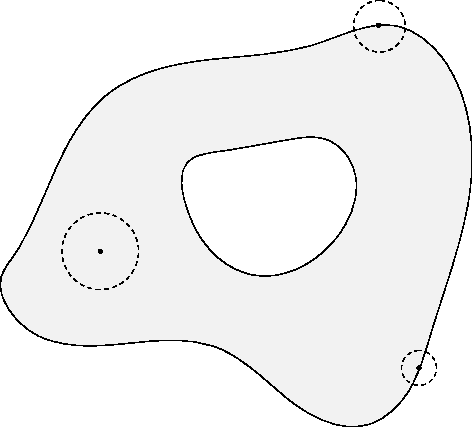
\includegraphics[scale=0.6]{fig/accumulation-pt.pdf}
	\caption{A few accumulation points of a set.}
\end{figure}


\begin{ex}[]
Discrete metric spaces have no accumulation points.
\end{ex}

\begin{prop}
	Every point in $A^o$ is an accumulation point of $A \subset \mathbb{R}^n$.
\end{prop}
\begin{proof}
	Let $x \in A^o$, then there exists $\varepsilon>0$ such that $D(x,\varepsilon) \subset A^o \subset A$. Then $(D(x,\varepsilon) \backslash \{x\}) \cap A$ is nonempty.
\end{proof}

\begin{prop}
	$A \subset (M,d)$ is closed if and only if the accumulation points of $A$ belong to $A$.
\end{prop}

If a set has no accumulation points, then it satisfies this condition and is thus closed.

\begin{defn}[]
	Let $A \subset (M,d)$, then the \textbf{closure} $\overline{A}$ of $A$ is the intersection of all closed sets containing $A$.
\end{defn}

\begin{prop}
	For $A \subset M$, $\bar{A}=A \cup \text{acc}(A)$.
\end{prop}

\begin{defn}[]
	The \textbf{boundary} of $A \subset (M,d)$ is $\partial A = \overline{A}\cap \overline{A^c}$.
\end{defn}
The union of 2 closed sets is closed, so $\partial A$ is closed. Note $\partial A = \partial A^c $.

\begin{prop}
	Let $A \subset M$, then $x \in \partial A$ if and only if for all $\varepsilon>0$, $D(x,\varepsilon)$ contains points of $A$ and $A^c$ (these points might include $x$ itself).
\end{prop}

\begin{ex}[]
	\begin{enumerate}
		\item Let $A=(0,1)$, then $\overline{A}=[0,1]$ and $\overline{A^c} =(-\infty,0] \cup[1,\infty)$. Then $\partial A = \{0,1\}$.
		\item Let $A=\mathbb{Q}$, then $\overline{A}=\mathbb{R}$. $A^c = \mathbb{R}\backslash \mathbb{Q}$, so $\overline{A_c} = \mathbb{R}$. Thus $\partial \mathbb{Q}=\mathbb{R}$.
	\end{enumerate}
\end{ex}

%%%%%%%%%%%%%%%%%%%%
% Compactness
%%%%%%%%%%%%%%%%%%%%

\section{Compactness}

\begin{defn}{Cover}{cover}
	A \textbf{cover} of $A \subset (M,d)$ is a collection $\left\{ U_i \right\}$ of sets whose union contains $A$. It is an \textbf{open cover} if each $U_i$ is open (in which case the union is always also open). A \textbf{subcover} of a given cover is a subcollection of $\left\{ U_i \right\}$ that covers $A$.
\end{defn}

\begin{defn}[]
	$A \subset (M,d)$ is \textbf{compact} if every open cover of $A$ has a finite subcover.
\end{defn}

\begin{prop}
Compact sets are closed and bounded.
\end{prop}

\begin{prop}
Closed subsets of compact sets are closed.
\end{prop}

\begin{defn}[]
	$A \subset (M,d)$ is \textbf{sequentially compact} if every sequence in $A$ has a subsequence that converges to a point in $A$.
\end{defn}

\begin{thrm}[Bolzano-Weierstrass]
	$A \subset (M,d)$ is compact if and only if $A$ is sequentially compact.
\end{thrm}

\begin{defn}[]
	$A$ is \textbf{totally bounded} if for every $\varepsilon>0$, there is a finite set \[\{ x_1,\dots,x_{N(\varepsilon)} \} \subset M\] such that \[A \subset \bigcup_{i=1}^{N(\varepsilon)} D(x_i,\varepsilon).\]
\end{defn}

\begin{prop}
Sequentially compact sets are totally bounded.
\end{prop}

\begin{thrm}[]
	$(M,d)$ is compact if and only if $M$ is complete and bounded. Similarly, $A \subset (M,d)$ is compact if and only if $A$ is closed and bounded.
\end{thrm}

\begin{thrm}[Heine-Borel]
	$A \subset \mathbb{R}^n$ is compact if and only if it is closed and bounded.
\end{thrm}

\begin{thrm}[Nested Set Property]
	Let $\left\{ F_k \right\}$ be a sequence of compact nonempty sets in a metric space $M$ such that $F_{k+1}\subset F_k$, then their intersection is nonempty, i.e.
	 \[
	\bigcap_{k=1}^\infty F_k \neq \varnothing.
	\] 
\end{thrm}

This can be inverted in a sense. Let $A_k = F_k^c$, then each $U_k$ is open and $U_{k+1} \supset U_k$. Then $\cup_{k=1}^\infty U_k \neq M$. Thus if $M$ is a metric space and the open sets $U_k$ are increasing and have compact complements, then the union of all the $U_k$'s is not all of $M$. 

\begin{figure}[H]
	\centering
	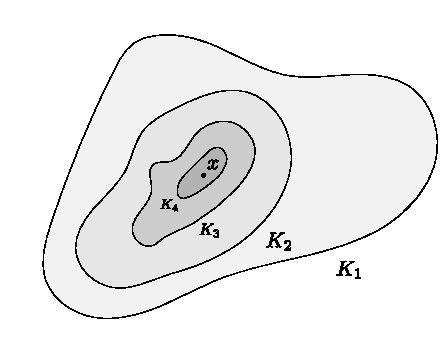
\includegraphics[scale=1]{fig/nested-set.pdf}
	\caption{As long as each $K_i$ is compact, $x$ is guaranteed to exist}
\end{figure}

%%%%%%%%%%%%%%%%%%%%
% Connectedness
%%%%%%%%%%%%%%%%%%%%

\section{Connectedness}

\begin{defn}[]
	A map $\phi:[a,b]\to M$ is \textbf{continuous} if $t_k \to t$ implies $\phi(t_k) \to \phi(t)$ for every sequence $\left\{ t_k \right\} \subset [a,b]$ converging to some $t \in [a,b]$.
\end{defn}

\begin{defn}[]
	A \textbf{path} joining two points $x $ and $y$ in $M$ is a continuous map $\phi:[a,b] \to M$ such that $\phi(a)=x, \phi(b)=y$. A set is \textbf{path-connected} if every two points in the set can be joined by a path lying in the set.
\end{defn}

A path-connected set need not be open or closed. Consider $[0,1], (0,1)$, and $[0,1)$, which are all connected.

\begin{defn}[]
	Let $A \subset (M,d)$, then two open sets $U,V$ \textbf{separate} $A$ if
	\begin{enumerate}
		\item $U \cap V \cap A = \varnothing$,
		\item $A \cap U \neq \varnothing$,
		\item $A \cap V \neq \varnothing$, and
		\item $A \subset U \cup V$.
	\end{enumerate}
	$A$ is \textbf{disconnected} if such sets exist, and it is \textbf{connected} if no such sets exist.
\end{defn}

\begin{figure}[H]
	\centering
	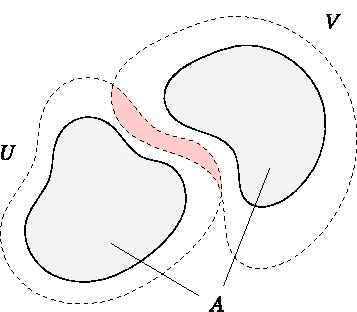
\includegraphics[scale=1]{fig/disconnected.pdf}
	\caption{A disconnected set.}
\end{figure}

\begin{prop}
	$[a,b]$ is connected.
\end{prop}

\begin{thrm}[]
Path-connected sets are connected.
\end{thrm}

\begin{defn}[]
	A \textbf{component} of a set $A$ is a maximal connected subset of $A$. A \textbf{path component} is a maximal path-connected subset of $A$.
\end{defn}

%+-------------------+
%| +---------------+ |
%| |    Chapter    | |
%| +---------------+ |
%+-------------------+
% Sequences and Series

\chapter{Sequences and Series}

%%%%%%%%%%%%%%%%%%%%
% Sequences and Limits
%%%%%%%%%%%%%%%%%%%%

\section{Sequences and Limits}

\begin{defn}[]
	A function $f:\mathbb{N} \to S$ is a \textbf{sequence} in $S$. A \textbf{subsequence} in $S$ is a function $f \circ \sigma$, where $\sigma:\mathbb{N}\hookrightarrow \mathbb{N}$ is injective and increasing.
\end{defn}

\begin{defn}[]
	A sequence $\left\{ x_n \right\}_{n=1}^\infty \subset (M,d)$ \textbf{converges} to $L \in M$ if for every neighborhood $U$ of $L$, there exists $N$ such that $x_n \in U$ when $n > N$.
\end{defn}


\begin{prop}[Squeeze Lemma]
	If $x_n \to L$ and $z_n \to L$ and $x_n \leq y_n \leq z_n$ for any $n > n_0$, then $y_n \to L$.
\end{prop}

\begin{prop}
	Limits are unique in an Archimedean field.
\end{prop}

\begin{thrm}
Let $x_n \to x$ and $y_n \to y$, then
\begin{enumerate}
	\item $x_n + y_n \to x+y$
	\item $\lambda x_n \to \lambda x$
	\item $x_n y_n \to xy$ 
	\item $y_n \neq 0, y \neq 0 \implies x_n y_n^{-1} \to xy^{-1}$
\end{enumerate}
\end{thrm}

\begin{defn}
	Let $F$ be an ordered field. We say that $F$ has the \textbf{Monotone Sequence Property} if every monotone nondecreasing sequence bounded above converges. An ordered field is \textbf{complete} if it has the Monotone Sequence Property.
\end{defn}

Complete ordered fields are Archimedean.

\begin{ex}[]
	For the discrete metric, a sequence $\left\{ x_n \right\}$ converges if and only if it is eventually constant.
\end{ex}

\begin{prop}
	$F\subset (M,d)$ is closed if an only if for all sequences in $F$ that converge to a point in $M$, that point is also in $F$.
\end{prop}

\begin{prop}
	For a set $A \subset (M,d)$, $x \in \overline{A}$ if and only if there is a sequence $x_k \in A$ with $x_k \to x$.
\end{prop}

\begin{ex}[]
	Consider the open interval $(0,1)$ with the usual metric. The sequence $\left\{ 1/n \right\}$ does \textit{not} converge in this metric space since $0 \not\in M$.
\end{ex}

\begin{prop}
	$v_k \to v$ in $\mathbb{R}^n$ if and only if each sequence of coordinates converges to the corresponding coordinate of $v$ as a sequence in $\mathbb{R}$.
\end{prop}

\section{Infimums and Supremums}

\begin{defn}[]
	The \textbf{supremum} of a set $S \subset \mathbb{R}$ is the least upper bound of $S$, and the \textbf{infimum} is the greatest upper bound.
\end{defn}

Least upper bounds are unique. If $b$ is an upper bound of $S$ and $b \in S$, then $b$ is the least upper bound.

\begin{prop}
	Let $S \subset \mathbb{R}$ be nonempty. Then $b \in \mathbb{R}$ is the least upper bound of $B$ if and only if $b$ is an upper bound of $S$ and for every $\varepsilon > 0$ there is an $x \in S$ such that $x > b-\varepsilon$.
\end{prop}

\begin{prop}
	Let $A \subset B \subset \mathbb{R}$, then $\inf B \leq \inf A \leq \sup A \leq \sup B$.
\end{prop}

\begin{thrm}{}{}
	In $\mathbb{R}$ the following hold
	\begin{enumerate}
		\item Least upper bound property: Let $S \subset \mathbb{R}$ be non-empty and have an upper bound, then $S$ also has a least upper bound.
		\item Greatest lower bound property: Let $S \subset \mathbb{R}$ be non-empty and have a lower bound, then $S$ also has a greatest lower bound.
	\end{enumerate}
\end{thrm}
This theorem is equivalent to the completeness axiom for ordered fields.


%%%%%%%%%%%%%%%%%%%%
% Limit Inferiors and Limit Superiors
%%%%%%%%%%%%%%%%%%%%

\section{Limit Inferiors and Limit Superiors}
\begin{defn}[]
Let $\left\{ x_n \right\}_{n=1}^\infty \subset \mathbb{R}$ be bounded above, then we define the \textbf{limit superior} to be
\[
	L = \overline{\lim} \;x_j = {\lim\sup}_{j\to\infty}x_j.
\] Similarly, define the \textbf{limit inferior} to be
\[
	\underline{\lim} \;x_j = {\lim\inf}_{j\to\infty} x_j.
\] 
\end{defn}

The limit inferior need not be the infimum, and the limit supremum need not be the supremum. The limit inferior is the limit of the infimums if we keep removing elements from the beginning of the sequence, and the limit superior is the limit of the supremums.

\begin{prop}
	Let $\left\{ x_n \right\}$ be a sequence in $\mathbb{R}$.
	\begin{enumerate}
		\item If $\left\{ x_n \right\}$ is bounded below, a number $a$ is equal to the limit inferior if and only if
			\begin{enumerate}
				\item For all $\varepsilon>0$, there exists $N$ such that $a-\varepsilon<x_n$ when $n>N$, and
				\item For all $\varepsilon>0$ and for all $M$, there exists $n > M$ with $x_n < a + \varepsilon$.
			\end{enumerate}

		\item If $\left\{ x_n \right\}$ is bounded above, a number $b$ is equal to the limit superior if and only if
			\begin{enumerate}
				\item For all $\varepsilon>0$, there exists $N$ such that $x_n < b + \varepsilon$ when $n >N$, and
				\item For all $\varepsilon>0$ and for all $M$, there exists $n > M$ with $b-\varepsilon< x_n$.
			\end{enumerate}
	\end{enumerate}
\end{prop}

%%%%%%%%%%%%%%%%%%%%
% Cauchy Sequences
%%%%%%%%%%%%%%%%%%%%

\section{Cauchy Sequences}

\begin{defn}[]
	The sequence $\left\{ x_n \right\}\subset (M,d)$ is a \textbf{Cauchy sequence} if for all $\varepsilon>0$, there exists $N$ such that if $n,m>N$, then $d(x_n,x_m) < \varepsilon$.
\end{defn}

\begin{defn}[]
	A metric space $(M,d)$ is \textbf{complete} if every Cauchy sequence in $M$ converges.
\end{defn}

\begin{ex}[]
	\begin{enumerate}
		\item $\mathbb{R}^n$ is complete.
		\item Any discrete metric space is complete.
	\end{enumerate}
\end{ex}

\begin{defn}[]
	$A \subset (M,d)$ is \textbf{bounded} if there exists some $p \in M$ and $R>0$ such that $A \subset D(p,R)$.
\end{defn}

\begin{figure}[H]
	\centering
	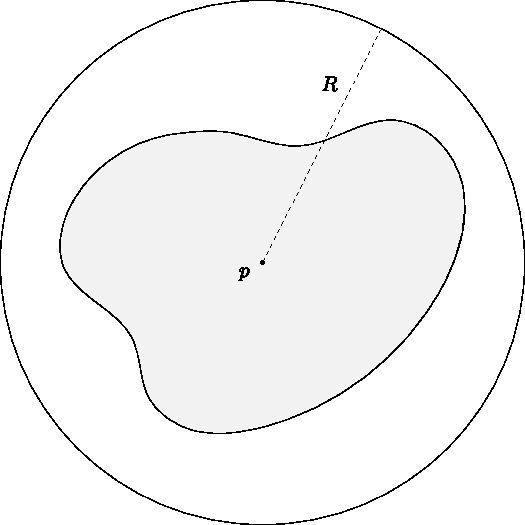
\includegraphics[scale=0.6]{fig/bounded.pdf}
	\caption{A bounded set}
\end{figure}

\begin{prop}
	A convergent sequence in a metric space is bounded.
\end{prop}

\begin{prop}
	\begin{enumerate}
		\item Every convergent sequence in a metric space is a Cauchy sequence.
		\item A Cauchy sequence in a metric space is bounded.
		\item If a subsequence of a Cauchy sequence converges to $x$, then the sequence converges to $x$.
	\end{enumerate}
\end{prop}

\begin{thrm}{}{}
	A sequence $\left\{ x_k \right\} \subset \mathbb{R}^n$ converges to a point in $\mathbb{R}^n$ if and only if it is a Cauchy sequence.
\end{thrm}

\begin{thrm}[Bolzano-Weierstrass Property]
	Every bounded sequence in $\mathbb{R}$ has a subsequence that converges to some point in $\mathbb{R}$.
\end{thrm}

Thus a sequence of points in $[a,b]$ has a subsequence that converges to a point in $[a,b]$.

\begin{thrm}[]
	Every Cauchy sequence in $\mathbb{R}$ converges to an element of $\mathbb{R}$.
\end{thrm}
\begin{proof}
Every Cauchy sequence is bounded, so by the Bolzano-Weierstrass property, every Cauchy sequence has a subsequence that converges to some point in $\mathbb{R}$. But if a subsequence of a Cauchy sequence converges to a point, then the sequence itself converges to that point. Thus every Cauchy sequence converges to a point in $\mathbb{R}$.
\end{proof}

%%%%%%%%%%%%%%%%%%%%
% The Real Numbers
%%%%%%%%%%%%%%%%%%%%

\section{The Real Numbers}

\begin{thrm}[]
	There's a unique (up to isomorphism) complete ordered field called the real number system. It is constructed as follows:
	Let $S$ be defined
	\[
		S = \left\{ (x_1, x_2, \dots) | x_n \in \mathbb{Q} \text{, sequence is increasing and bounded above} \right\}
	\] 
	and let two members of $S$ be equivalent if their upper bounds are the same. Then $\mathbb{R}$ is the set of all equivalence classes in $S$. We do not include $\pm \infty$ in $\mathbb{R}$.
\end{thrm}

\begin{prop}
$\mathbb{Q}$ is dense in $\mathbb{R}$.
\end{prop}

Although $\mathbb{Q}$ is dense in $\mathbb{R}$, there are actually many more irrationals than rationals.

\begin{prop}[]
	The interval $(0,1)$ in $\mathbb{R}$ is uncountable.
\end{prop}

Since the function $f(x) = a + (b-a)x$ maps $]0,1[ \mapsto ]a,b[$, any interval in $\mathbb{R}$ is uncountable. Since $\mathbb{R}$ is uncountable but $\mathbb{Q}$ is countable, it must be the case that $\mathbb{C}$ is uncountable.

\section{Norms and Inner Products}

\begin{defn}[]
	A \textbf{normed vector space} $(\mathcal{V}, \Vert{\cdot}\Vert)$ is a vector space $\mathcal{V}$ and a function $\Vert{\cdot}\Vert:\mathcal{V}\to\mathbb{R}$ such that
	\begin{enumerate}
		\item $\Vert{v}\Vert\geq 0$ 
		\item $\Vert{v}\Vert=0 \iff v=0$
		\item $\Vert{\lambda v}\Vert=|\lambda| \Vert{v}\Vert$ 
		\item $\Vert{v+w}\Vert\leq \Vert{v}\Vert+\Vert{w}\Vert$
	\end{enumerate}
\end{defn}

\begin{prop}
	If $(\mathcal{V},\Vert{\cdot}\Vert)$ is a normed vector space and $\left\{ v_k \right\}, \left\{ w_k \right\} \subset \mathcal{V}$ such that $v_k \to v$ and $w_k \to w$, and if $\left\{ \lambda_k \right\} \subset \mathbb{R}$ such that $\lambda_k \to \lambda$, then
	\begin{enumerate}
		\item $v_k + w_k \to v+w$
		\item $\lambda_k v_k \to \lambda v$
	\end{enumerate}
\end{prop}

Thus $w_k \to w \iff w_k - w \to 0$ for all sequences in normed vector spaces.


Norms always produce metrics, since we can define a metric $d(v,w)=\Vert{v-w}\Vert$ on any normed vector space; however, not all metrics (e.g. discrete or bounded metrics) can be produced from norms.

\begin{defn}[]
	An \textbf{inner product space} is a real vector space $\mathcal{V}$ with a function $\left\langle \cdot,\cdot \right\rangle:\mathcal{V}\times\mathcal{V}\to\mathbb{R}$ such that
	\begin{enumerate}
		\item $\left\langle v,v \right\rangle\geq 0$ 
		\item $\left\langle v,v \right\rangle=0 \iff v=0$ 
		\item $\left\langle \lambda v,w \right\rangle= \lambda \left\langle v,w \right\rangle$ for all $\lambda \in \mathbb{R}$ 
		\item $\left\langle v,w+u \right\rangle=\left\langle v,w \right\rangle+\left\langle v,u \right\rangle$ 
		\item $\left\langle v,w \right\rangle=\left\langle v,w \right\rangle$
	\end{enumerate}
\end{defn}

Inner products always produce norms, since on any inner product space we can define a norm $\Vert{v}\Vert=\sqrt{\left\langle v,v \right\rangle}$.

Two useful identities that aren't hard to prove:
\begin{enumerate}
	\item $\left\langle \lambda v + \mu w, u \right\rangle=\lambda \left\langle v,u \right\rangle+\mu\left\langle w,u \right\rangle$ 
	\item $\left\langle 0,w \right\rangle=\left\langle w,0 \right\rangle=0$
\end{enumerate}

\begin{prop}[Cauchy-Schwarz Inequality]
	If $(\mathcal{V},\left\langle \cdot,\cdot \right\rangle)$ is an inner product space, then we have $|\left\langle v,w \right\rangle| \leq \sqrt{\left\langle v,v \right\rangle} \sqrt{\left\langle w,w \right\rangle}$ for all $v,w \in \mathcal{V}$.
\end{prop}

\begin{prop}[Triangle Inequality]
	$\Vert{x+y}\Vert^2 \leq \Vert{x}\Vert^2 + \Vert{y}\Vert^2$.
\end{prop}
\begin{proof}
	Cauchy-Schwarz gives
	\begin{align*}
		\Vert{x+y}\Vert^2 &= \Vert{x}\Vert^2 + 2\left\langle x,y \right\rangle + \Vert{y}\Vert^2 \\
				  &\leq \Vert{x}\Vert^2 + 2\Vert{x}\Vert\Vert{y}\Vert + \Vert{y}\Vert^2 \\
				  &= \Vert{x}\Vert^2 + \Vert{y}\Vert^2.
	\end{align*}
\end{proof}


%%%%%%%%%%%%%%%%%%%%
% Euclidean Space
%%%%%%%%%%%%%%%%%%%%

\section{Euclidean Space}

\begin{thrm}[]
	Euclidean $n$-space with addition and scalar multiplication is a vector space of dimension $n$.
\end{thrm}

The norm of $x \in \mathbb{R}^n$ is defined
\[
	|x| = \left( \sum_{i=1}^{n} x_i^2 \right)^{1/2}.
\] 

The distance between $x$ and $y$ is defined $d(x,y) = |x-y|$. The inner product is defined $\left\langle x,y \right\rangle = \sum_{i=1}^{n} x_i y_i$. Note that $|x|^2 = \left\langle x,x \right\rangle$.

\begin{prop}
	Let $v,w \in \mathbb{R}^n$, and let
	\[
		\rho(v,w) = \max \left\{ |v_1-w_1|, |v_2-w_2|, \dots, |v_n-w_n| \right\}.
	\]
	Then
	 \[
		 \rho(v,w) \leq \Vert{v-w}\Vert \leq \sqrt{n} \; \rho(v,w)
	\] 
\end{prop}

%%%%%%%%%%%%%%%%%%%%
% Series in Normed Vector Spaces
%%%%%%%%%%%%%%%%%%%%

\section{Series in Normed Vector Spaces}

Let $(\mathcal{V},|\cdot|)$ be a normed vector space and let $\left\{ x_i \right\}_{i=1}^\infty\subset \mathcal{V}$. Set $S_n \doteq \sum_{i=1}^{n} x_i$. If $S_n \to L$, we say $\sum_{i=1}^{\infty} x_i$ is convergent and $\sum_{i=1}^{\infty} x_i = L$. If $\left\{ S_n \right\}$ does \textit{not} converge, we say $\sum_{i=1}^{\infty} x_i$ does not converge.

If $\mathcal{V}=\mathbb{R}$, we say $S_i \to \infty$ if for all $M$, there exists $N$ such that if $n  >N$, then $S_n > M$. If $S_i \to \pm \infty$, we say $\sum_{i=1}^{\infty} x_i = \pm\infty$ (respectively).

\begin{defn}[]
A \textbf{Banach space} is a complete normed vector space. A \textbf{Hilbert space} is a complete inner product space.
\end{defn}

\begin{thrm}[]
	Let $\mathcal{V}$ be a complete normed vector space. A series $\sum x_k $ converges if and only if for every $\varepsilon>0$, there is an $N$ such that $k  >N$ implies
	\[
	\Vert{x_k + x_{k+1}+\cdots+x_{k+p}}\Vert<\varepsilon
	\] 
	for all integers $p=0,1,2,\dots$
\end{thrm}
\begin{proof}
	Let $s_k = \sum_{i=1}^{k} x_k$. Since $\mathcal{V}$ is complete, a $\left\{ s_k \right\}$ converges if and only if it is a Cauchy sequence. This is true if and only if there is an $N$ such that $l > N$ implies $\Vert{s_l - s_{l+q}}\Vert <\varepsilon$ for all $q=1,2,\dots$. But $\Vert{s_l - s_{l+q}}\Vert=\Vert{x_{l+1}+\cdots+x_{l+q}}\Vert$, and so the result follows with $k=l+1$ and $p=q-1$.
\end{proof}

\begin{thrm}{}{}
In a complete normed vector space, if $\sum x_k$ converges absolutely, then $\sum x_k$ converges.
\end{thrm}
\begin{proof}
	This follows from the previous theorem and the triangle inequality
	 \[
	\Vert{x_k + \cdots + x_{k+p}}\Vert \leq \Vert{x_k}\Vert+\cdots+\Vert{x_{k+p}}\Vert.
	\] 
\end{proof}

%+-------------------+
%| +---------------+ |
%| |    Chapter    | |
%| +---------------+ |
%+-------------------+
% Continuity, Differentiation, and Integration

\chapter{Continuity, Differentiation, and Integration}

%%%%%%%%%%%%%%%%%%%%
% Continuity
%%%%%%%%%%%%%%%%%%%%

\section{Continuity}

\begin{defn}[]
Let $f: A \subset M_1 \to M_2$. Suppose that $x_0$ is an accumulation point of $A$, then $b \in M_2$ is the \textbf{limit of $f$ at $x_0$} 
\[
	\lim_{x \to x_0} f(x) = b
\] 
if given any $\varepsilon>0$, there exists $\delta>0$ such that for all $x\in A$ satisfying $x_0 \neq x$ and $d_1(x,x_0)<\delta$, we have $d_2(f(x),b))<\varepsilon$.

Equivalently, there exists $\delta>0$ such that $f(D(x_0,\delta) \backslash \left\{ x_0 \right\}) \subset D(L,\varepsilon)$.
\end{defn}

The limit of a function at any given point need not exist, but when it does exist, it is unique.

\begin{defn}[]
Let $A \subset M_1$, $f:A \to M_2$, and $x_0 \in A$. We say that $f$ is continuous at $x_0$ if either $x_0$ is not an accumulation point of $A$ or $\lim_{x \to x_0} f(x)=f(x_0)$.
\end{defn}

\begin{thrm}[]
	Let $f:A \subset M_1 \to M_2$, then the following are equivalent.
\begin{enumerate}
	\item $f$ is continuous at every point of $A$.
	\item For every convergent sequence $x_k \to x$ in $A$, we have $f(x_k) \to f(x)$.
	\item For every open set $U \subset M_2$, $f^{-1}(U)$ is open in $M_1$.
	\item For every closed set $F \subset M_2$, $f^{-1}(F)$ is closed in $M_1$.
\end{enumerate}
\end{thrm}

\begin{figure}[H]
	\centering
	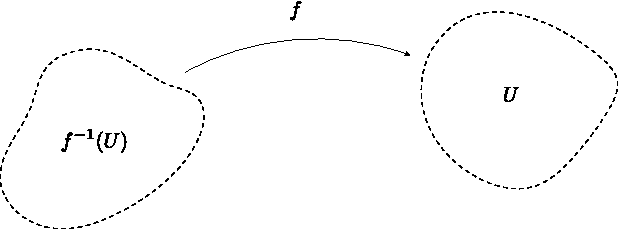
\includegraphics[scale=1]{fig/cts.pdf}
	\caption{A continuous function $f$.}
\end{figure}

\begin{thrm}[]
	The continuous image of a (path) connected set is (path) connected. The continuous image of a compact set is compact.
\end{thrm}

\begin{thrm}[Maximum-Minimum Theorem]
	Let $A \subset (M,d)$ be compact and suppose $f:A \to \mathbb{R}$ is continuous. Then $f$ is bounded on $K$ and attains its infimum and supremum on $K$.
\end{thrm}
\begin{proof}
	Since $K$ is compact and $f$ is continuous, $f(K)$ is compact, so it is also closed and bounded. Since it's closed, it contains its accumulation points. Its infimum and supremem are either in the set or accumulation points, so they must lie in $f(K)$.
\end{proof}

\begin{prop}
	Compositions of continuous functions are continuous.
\end{prop}

\begin{prop}
	If $(M,d)$ is a metric space, $\mathcal{V}$ is a normed vector space, and $f:M\to \mathcal{V}$, $g:M\to \mathcal{V}$, and $h:M \to \mathbb{R}$ are continuous, then
	\begin{enumerate}
		\item $f+g$ is continuous, and
		\item $hf$ is continuous.
	\end{enumerate}
\end{prop}

\begin{thrm}[Intermediate Value Theorem]
	Let $A \subset (M,d)$, and let $f:A \to \mathbb{R}$ be continuous. Suppose that $K \subset A$ is connected and $x,y \in K$. Then for every real number $c \in \mathbb{R}$ such that $f(x) < c < f(y)$, there exists a point $z \in K$ such that $f(z) = c$.
\end{thrm}
\begin{proof}
	Suppose no such $z$ exists, then $f(A) \subset (-\infty,c) \cup (c, \infty)$. Since $y_1 < c$ and $y > c$, we know both sets in this union are nonempty. Since $f(A)$ is then clearly covered by two disjoint nonempty sets, it is disconnected. Since $A$ was taken to be path-connected (and thus also connected), this is a contradiction, so such a $z$ actually does exist.
\end{proof}

\begin{figure}[H]
	\centering
	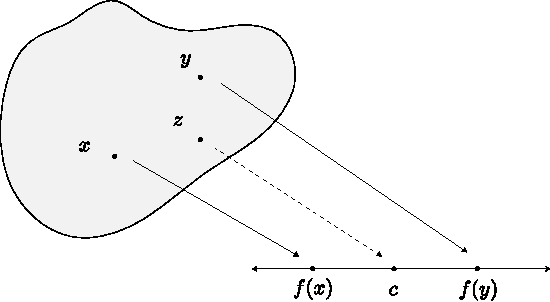
\includegraphics[scale=0.8]{fig/intermediate-value.pdf}
	\caption{The Intermediate Value Theorem.}
\end{figure}


%%%%%%%%%%%%%%%%%%%%
% Uniform Continuity
%%%%%%%%%%%%%%%%%%%%

\section{Uniform Continuity}
\begin{defn}[]
	$f:M_1 \to M_2$ is \textbf{uniformly continuous} if for all $\varepsilon>0$ and for all $x,y \in M_1$, there exists $\delta>0$ such that if $d_1(x,y) < \delta$, then $d_2(f(x), f(y)) < \varepsilon$.
\end{defn}

It should be clear how to restrict the uniform continuity of $f$ to certain subsets of $M_1$.

Note that unlike usual continuity, we have to find a $\delta$ that works for \textit{all} $x$ and $y$, so it must be independent of the inputs to the function.

\begin{thrm}[]
Let $f:M_1\to M_2$ be continuous and let $K \subset M_1$ be compact, then $f$ is uniformly continuous on $K$.
\end{thrm}

%%%%%%%%%%%%%%%%%%%%
% Differentiation of Functions of One Variable
%%%%%%%%%%%%%%%%%%%%

\section{Differentiation of Functions of One Variable}
\begin{defn}[]
The \textbf{derivative} of a function $f$ at point $x$ is defined
\[
	f'(x) \doteq \lim_{h \to 0} \frac{f(x+h)-f(x)}{h}.
\] 
\end{defn}

We can rewrite the definition for differentiability that avoids the issue of division by a term that approaches 0: for any $\varepsilon>0$, there is a $\delta>0$ such that if $|\Delta x|< \delta$, then
\[
	|f(x + \Delta x) - f(x) - f'(x) \Delta x| \leq \varepsilon |\Delta x|.
\] 

\begin{defn}[]
	Let $\phi,g:(0,a) \to \mathbb{R}$. We say $\phi$ is $\mathcal{O}(g)$ if
	 \[
		 \left|\frac{\phi(x)}{g(x)} \right|
	 \] is bounded in some ``deleted'' neighborhood of 0, i.e. it lies in $D(0,r)\backslash\left\{ 0 \right\}$ for some $r>0$. Additionally, we say $\phi$ is $o(g)$ if \[\lim_{x \to 0} \frac{\phi(x)}{g(x)} = 0.\]
\end{defn}

Based on these definitions, we can see that $f$ is differentiable at $x$ if there exists some $L \in \mathbb{R}$ such that $f(y)-f(x)-L(y-x)$ is $o(|y-x|)$.

\begin{defn}[]
	A function $f:M_1\to M_2$ is \textbf{Lipschitz} if there exists some $L \geq 0$ such that $d_2(f(x), f(y)) \leq L d_1(x,y)$ for all $x,y \in M_1$. The function $f$ is \textbf{locally Lipschitz} if for every compact set $K \subset M_1$, $f$ restricted to $K$ is Lipschitz.
\end{defn}

Lipschitz functions are also uniformly continuous. If we want $d_2(f(x),f(y))$ be to less than some $\varepsilon>0$, then choose $x$ and $y$ such that $d_1(x,y) < \varepsilon/L$.

\begin{prop}
	If $f$ is differentiable at $x$, then $f$ is continuous at $x$.
\end{prop}

\begin{thrm}{}{}
Suppose that $f$ and $g$ are differentiable at $x$ and that $k \in \mathbb{R}$, then $kf$, $f+g$, and $fg$ are differentiable at $x$ and
\begin{enumerate}
	\item $(kf)'(x) = kf'(x)$,
	\item $(f+g)'(x) = f'(x) + g'(x)$, and
	\item $(fg)'(x) = f'(x) g(x) + f(x) g'(x)$.
\end{enumerate}
\end{thrm}

\newpage
\begin{thrm}[Chain Rule]
	If $f$ is differentiable at $x$ and $g$ is differentiable at $f(x)$, then $g \circ f$ is differentiable at $x$ and
	\[
		(g \circ f)'(x) = g'(f(x)) f'(x).
	\] 
\end{thrm}

\begin{defn}[]
If $f^{(n-1)}$ is differentiable and $f^{(n)}$ continuous, $f$ is $C^{n}$. The function $f$ is $C^{\infty}$ if it is infinitely differentiable. 
\end{defn}

\begin{defn}[]
	A function $f$ defined in a neighborhood of $x$ is \textbf{increasing} at $x$ if there is an interval $(a,b)$ containing $x$ such that
	\begin{enumerate}
		\item If $a < y < x$, then $f(y) \leq f(x)$, and
		\item If $x < y < b$, then $f(y) \geq f(x)$.
	\end{enumerate}
	The notions of decreasing and strictly increasing/decreasing functions are similar.
\end{defn}

\begin{thrm}[]
Let $f$ be differentiable at $x$, then
\begin{enumerate}
	\item If $f$ is increasing at $x$, then $f'(x) \geq 0$,
	\item If $f$ is decreasing at $x$, then $f'(x) \leq 0$,
	\item If $f'(x) > 0$, then $f$ is strictly increasing at $x$, and
	\item If $f'(x) < 0$, then $f$ is strictly decreasing at $x$.
\end{enumerate}
\end{thrm}

\begin{prop}
	If $f:(a,b) \to \mathbb{R}$ is differentiable at $c \in (a,b)$ and if $f$ has a maximum (or minimum) at $c$, then $f'(c) = 0$.
\end{prop}
\begin{proof}
	If $f'(c) > 0$, then $f$ is strictly increasing at $c$, which is a contradiction. If $f'(c) < 0$, then $f$ is strictly decreasing at $c$, which is also a contradiction. Thus $f'(c)=0$.
\end{proof}

\begin{thrm}[Rolle's]
	If $f:[a,b] \to \mathbb{R}$ is continuous, $f$ is differentiable on $(a,b)$, and $f(a) = f(b) = 0$, then there is a number $c \in (a,b)$ such that $f'(c) = 0$.
\end{thrm}

\begin{thrm}[Mean Value Theorem]
	If $f:[a,b] \to \mathbb{R}$ is continuous and differentiable on $(a,b)$, there is a point $c \in (a,b)$ such that $f(b) - f(a) = f'(c) (b-a)$.
\end{thrm}
\begin{proof}
	Let \[\varphi(x) = f(x)-f(a)-(x-a)\frac{f(b)-f(a)}{b-a}, \]
	then apply Rolle's Theorem.
\end{proof}

\begin{figure}[H]
	\centering
	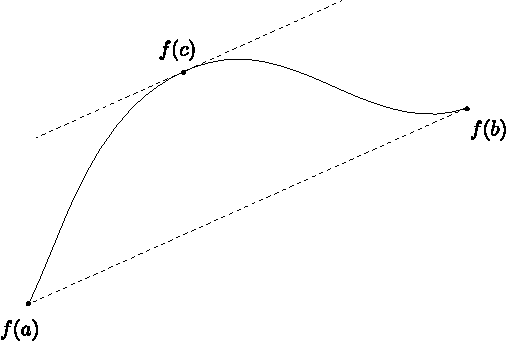
\includegraphics[scale=0.7]{fig/mean-value.pdf}
	\caption{The Mean Value Theorem.}
\end{figure}


\begin{cor}
	If $f:[a,b] \to \mathbb{R}$ is continuous and $f'=0$ on $(a,b)$, then $f$ is constant.
\end{cor}
\begin{proof}
	Applying the mean value theorem to $f$ gives a point $c$ such that $f(b)-f(a) = f'(c)(b-a) = 0$, so $f(a) = f(b)$ for all $x \in [a,b]$. Thus $f$ is constant.
\end{proof}

\begin{cor}
	If $f:(a,b)\to\mathbb{R}$ is differentiable with $|f'(x)|\leq M$ for every $x \in (a,b)$, then $f$ is $M$-Lipschitz.
\end{cor}

\begin{prop}
	Let $f \in C([a,b])$ be differentiable on $(a,b)$ such that $f'(x) \geq 0$ for every $x \in (a,b)$, then $f$ is increasing on $[a,b]$. If $f'(x) \leq 0$ for every $x \in(a,b)$ instead, then $f$ is decreasing on $[a,b]$.
\end{prop}

\begin{thrm}[Inverse Function Theorem]
	Suppose $f:(a,b) \to \mathbb{R}$ is strictly monotonic over $(a,b)$. Then $f$ is a bijection onto its range, $f^{-1}$ is differentiable on its domain, and $(f^{-1})'(y) = 1/f'(x)$ where $f(x) = y$.
\end{thrm}

\begin{prop}
	Suppose that $f$ is continuous on $[a,b]$ and twice differentiable on $(a,b)$ and that $x \in (a,b)$, then
	\begin{enumerate}
		\item If $f'(x) = 0$ and $f''(x) > 0$, then $x$ is a strict local minimum of $f$, and
		\item If $f'(x) = 0$ and $f''(x) < 0$, then $x$ is a strict local maximum of $f$.
	\end{enumerate}
\end{prop}

%%%%%%%%%%%%%%%%%%%%
% Integration of Functions of One Variable
%%%%%%%%%%%%%%%%%%%%

\section{Integration of Functions of One Variable}

The integral of a function of one variable is the signed area under the curve. To define these, we'll need a notion of partitions and upper and lower sums.

\begin{defn}[]
The \textbf{mesh} of a partition $P =\left\{ x_1,x_2,\dots,x_N \right\}$ is defined
\[
	|P| \doteq \sup_i |x_{i+1}-x_i|.
\] 
\end{defn}

\begin{defn}[]
	Let $P$ and $Q$ be partitions of $[a,b]$. We say $P$ is a \textbf{refinement} of $Q$ if $Q \subset P$. We denote this by $Q \prec P$ or $P \succ Q$.
\end{defn}

Consider a bounded function $f:A \subset \mathbb{R}\to\mathbb{R}$. If $A$ is bounded, then there is some $[a,b]\supset A$. Define $f(x)=0$ if $x \in [a,b]\backslash A$. Now partition $[a,b]$ with $P=\left\{ x_0=a,x_1,\dots,x_n=b \right\}$ such that $x_0<x_1<\cdots<x_n$.

\begin{defn}{Upper/Lower Sums}{}
	The \textbf{upper sum} of $f$ over $P$ is
	\[
		U(f,P) = \sum_{i=0}^{n-1} \sup_{x\in[x_i,x_{i+1}]} f(x) (x_{i+1}-x_i).
	\] 
	Similarly, the \textbf{lower sum} is defined
	\[
		L(f,P) = \sum_{i=0}^{n-1} \inf_{x\in[x_i,x_{i+1}]} f(x) \cdot (x_{i+1}-x_i).
	\] 
\end{defn}

Note that the supremum and infimum for each subinterval exist since $f$ is bounded. Let $-M \leq f \leq M$, then
\[
	-M(b-a) \leq L(f,P) \leq U(f,P) \leq M(b-a)
\] for any partition $P$ of $[a,b]$.

\begin{prop}
	If $P \succ Q$, then $L(f,Q) \leq L(f,P) \leq U(f,P) \leq U(f,Q)$.
\end{prop}

Let $P$ and $Q$ be two partitions, then neither is necessarily a subset of the other. To get around this, we note that for all $P$ and $Q$, there exists a partition $R$ which refines both, i.e. $R \succ P$ and $R \succ Q$. The set $P \cup Q$ arranged into an ordered set is one such partition.

\newpage
\begin{defn}[]
Given a bounded function $f:A \to \mathbb{R}$ over a bounded set $A$, define the \textbf{upper integral} by
\[
	\overline{\int_{A} } f = \inf\left\{ U(f,P) \right\}_P
\] 
and the \textbf{lower integral} by
\[
	\underline{\int_{A} } f = \sup \left\{ L(f,P) \right\}_P.
\] 
\end{defn}

\begin{defn}[]
	A function $f$ is \textbf{Riemann integrable} if $\overline{\int_{A} } f = \underline{\int_{A} } f$. The common value $\overline{\int_{A} } f = \underline{\int_{A} } f$ is denoted by $\int_{A} f$. If $A=[a,b]$, we write
	\[ 
	\int_{A} f = \int_{a}^{b} f.
	\] 
\end{defn}

Note that this definition does \textit{not} involve any notions of smoothness or continuity.

\begin{thrm}{}{}
	Any non-increasing or non-decreasing function on $[a,b]$ is Riemann integrable on $[a,b]$.
\end{thrm}

\begin{thrm}{}{}
	If $f:[a,b]\to\mathbb{R}$ is bounded and continuous at all but finitely many points of $[a,b]$, then it is Riemann integrable on $[a,b]$.
\end{thrm}

\begin{prop}
	\label{prop:integral-props}
	Let $f$ and $g$ be Riemann integrable on $[a,b]$, then
	\begin{enumerate}
		\item If $k\in\mathbb{R}$, then $kf$ is integrable on $[a,b]$ and $\int_{a}^{b} kf = k \int_{a}^{b} f$,
		\item $f+g$ is integrable on $[a,b]$ and $\int_{a}^{b} (f+g)=\int_{a}^{b} f+\int_{a}^{b} g$,
		\item If $f(x) \leq g(x)$ for all $x \in [a,b]$, then $\int_{a}^{b} f \leq \int_{a}^{b} g$, and
		\item If $f$ is also integrable on $[b,c]$, then it is integrable on $[a,c]$ and $\int_{a}^{c} f = \int_{a}^{b} f + \int_{b}^{c} f$.
	\end{enumerate}
\end{prop}

\begin{cor}
	The absolute value of a definite integral of $f$ is a lower bound of the definite integral of the absolute value of $f$:
	\[
		\left| \int_{a}^{b} f(x) \;dx \right| \leq \int_{a}^{b} |f(x)| \;dx.
	\] 
\end{cor}

\newpage
\begin{prop}
	The lower definite integral of $f$ is a lower bound of the upper definite integral, i.e.
	\[
		\underline{\int_{a}^{b}} f(x) \;dx \leq \overline{\int_{a}^{b} } f(x) \;dx.
	\] 
\end{prop}

\begin{defn}[]
	An \textbf{antiderivative} of $f:[a,b] \to \mathbb{R}$ is a continuous function $F:[a,b]\to\mathbb{R}$ such that $F$ is differentiable on $(a,b)$ and $F'(x)=f(x)$ for $x\in(a,b)$.
\end{defn}

\begin{thrm}[The Fundamental Theorem of Calculus]
	Let $f:[a,b]\to\mathbb{R}$ be continuous, then $f$ has an antiderivative $F$ and
	\[
		\int_{a}^{b} f(x) \;dx = F(b)-F(a).
	\] 
	If $G$ is any other antiderivative of $f$, then we also have $\int_{a}^{b} f = G(b)-G(a)$.
\end{thrm}

%+-------------------+
%| +---------------+ |
%| |    Chapter    | |
%| +---------------+ |
%+-------------------+
% Uniform Convergence

\chapter{Uniform Convergence}

%%%%%%%%%%%%%%%%%%%%
% Pointwise and Uniform Convergence
%%%%%%%%%%%%%%%%%%%%

\section{Pointwise and Uniform Convergence}

\begin{defn}[]
	Let $X$ be a set and $M$ be a metric space. A sequence of functions $f_k : X \to M$ \textbf{converges pointwise} to $f:X \to M$ if for all $x \in X$, $f_k(x) \to f(x)$.
\end{defn}

Pointwise convergence is straightforward, but it might not preserve the properties of the $f_k$. As we can see in the next example, continuity of each $f_k$ need not translate to continuity of $f$ if we only have pointwise convergence.

\begin{ex}{}{}
Consider the sequence of sigmoid-like functions
\[
	f_k(x) = \frac{1}{1+e^{-kx}} .
\] As $k$ increases, the ``slope" of the curve near 0 gets steeper, getting closer to a vertical line. Each $f_k$ is continuous, but the sequence converges pointwise to
\[
	f(x) =
	\begin{cases}
		0 & x < 0 \\
		1/2 & x=0 \\
		1 & x>0,
	\end{cases}
\] which is clearly not continuous.
\end{ex}

\begin{defn}[]
	Suppose $f_k : X \to M$ is a sequence of functions such that for all $\varepsilon>0$, there is a $K$ such that $d(f_k(x), f(x)) < \varepsilon$ for all $x \in X$ when $k > K$. Then we say that $f_k$ \textbf{converges uniformly} to $f$.
\end{defn}

With uniform convergence, we have a bound on how slowly each $f_k(x)$ converges to its particular $f(x)$. As you might expect, this results in the preservation of more properties of the $f_k$. As we'll see later, if each $f_k$ is continuous or differentiable, then $f$ is continuous or differentiable, respectively.

\begin{figure}[H]
	\centering
	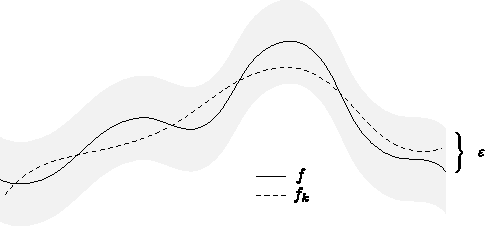
\includegraphics[scale=1.3]{fig/uniform-convergence.pdf}
\end{figure}

\begin{note}[]
	When $X$ is finite, both pointwise and uniform convergence are equivalent. Fix $\varepsilon>0$, then each $x_i$, there is a $K_i$ such that $|f(x_i) - f_k(x_i) | < \varepsilon$ when $k > K_i$. Since $X$ is finite, we can let $K = \max_i K_i$, then we clearly have uniform convergence.
\end{note}

\begin{defn}[]
	Let $g_k : X \to \mathcal{V}$ be a sequence of functions, where $\mathcal{V}$ is a normed vector space. We say $\sum_{k=1}^{\infty} g_k$ \textbf{converges pointwise} to $g:X \to \mathcal{V}$ if the sequence $s_n \doteq \sum_{k=1}^{n} g_k$ converges pointwise to $g$.

	Similarly, we say $\sum_{k=1}^{\infty} g_k$ \textbf{converges uniformly} to $g$ if $s_k$ converges uniformly to $g$.
\end{defn}

Note that in the above definition, we needed addition of our space's elements to make sense in order to talk about series, thus we used $\mathcal{V}$ instead of $M$.

\begin{prop}
	Let $f_k: M_1 \to M_2$ be a sequence of continuous functions, and let $f_k$ converge uniformly to $f$. Then $f$ is continuous on $M_1$.
\end{prop}

\begin{cor}
	Let $g_k: X \to \mathcal{V}$ be continuous for all $k$. If $\sum_{k=1}^{\infty} g_k$ converges uniformly to $g$, then $g$ is continuous.
\end{cor}
\begin{proof}
	This follows from the previous proposition and the fact that the sum of continuous functions is continuous (so each partial sum is continuous).
\end{proof}

\begin{note}[]
In other words, we can exchange limits with summations when the convergence is uniform, i.e.
\[
	\lim_{x \to x_0} \sum_{k=1}^{\infty} g_k(x) = \sum_{k=1}^{\infty} \lim_{x \to x_0} g_k(x).
\] 
\end{note}


%%%%%%%%%%%%%%%%%%%%
% The Weierstrass-M Test
%%%%%%%%%%%%%%%%%%%%

\section{The Weierstrass-M Test}

\begin{thrm}[Cauchy Criterion]
	Let $M$ be a complete metric space, $X$ a set, and $f_k: X \to M$ a sequence of functions. Then $f_k$ converges uniformly on $X$ if and only if for all $\varepsilon > 0$, there is a $K$ such that $d(f_k(x), f_l(x)) < \varepsilon$ for all $x \in X$ when $k,l > K$.
\end{thrm}

The Cauchy criterion can easily be rewritten to apply to series of functions instead: Let $\mathcal{V}$ be a Banach space, then $\sum_{k=1}^{\infty} g_k$ converges uniformly on $X$ if and only if for all $\varepsilon>0$, there is a $K$ such that
\[
	\Vert{g_k(x) + \cdots + g_{k+p}(x)}\Vert< \varepsilon
\] for all $x \in X$ and for all integers $p \geq 0$.

\begin{thrm}[Weierstrass-$M$ Test]
	Let $\mathcal{V}$ be a Banach space, and let $g_k : X \to \mathcal{V}$ with constants $M_k$ such that
	\[
		\Vert{g_k(x)}\Vert\leq M_k
	\] for all $x \in X$ and such that $\sum_{k=1}^{\infty} M_k$ converges. Then $\sum_{k=1}^{\infty} g_k$ converges uniformly (and absolutely).
\end{thrm}

%%%%%%%%%%%%%%%%%%%%
% Integration and Differentiation of Series
%%%%%%%%%%%%%%%%%%%%

\section{Integration and Differentiation of Series}

\begin{thrm}[]
	Let $f_k$ be Riemann integrable on $[a,b] $, and suppose that they converge uniformly to some function $f$ on $[a,b]$. Then $f$ is Riemann integrable on $[a,b]$ and
	\[
		\lim_{k \to \infty} \int_{a}^{b} f_k(x) \;dx = \int_{a}^{b} f(x)\;dx.
	\] 
\end{thrm}

\begin{cor}
	Let $g_k : [a,b] \to \mathbb{R}$ be Riemann integrable, and suppose $\sum_{k=1}^{\infty} g_k$ converges uniformly on $[a,b]$. Then
	\[
		\int_{a}^{b} \sum_{k=1}^{\infty} g_k = \sum_{k=1}^{\infty} \int_{a}^{b} g_k.
	\] 
\end{cor}
\begin{proof}
	Apply the previous theorem to the sequence of partial sums. We can do this because the sum of a finite number of Riemann integrable functions is itself Riemann integrable (see Proposition \ref{prop:integral-props}).
\end{proof}

\begin{thrm}{}{}
	Let $f_k:(a,b) \to \mathbb{R}$ be differentiable on $(a,b)$, and suppose that $f_k$ converges pointwise to $f:(a,b) \to \mathbb{R}$. Also suppose that $f_k'$ is continuous and converges uniformly to some $g$. Then $f$ is differentiable and $f'=g$.
\end{thrm}

\begin{cor}
	\label{cor:series-differentiation}
	Let $g_k$ be differentiable with $g_k'$ continuous, and suppose that $\sum_{k=1}^{\infty} g_k$ converges pointwise and $\sum_{k=1}^{\infty} g_k'$ converges uniformly, then
	\[
		\left( \sum_{k=1}^{\infty} g_k \right)' = \sum_{k=1}^{\infty} g_k'.
	\] 
\end{cor}

\begin{ex}{}{}
	Consider \[ \frac{1}{1-x} = \sum_{k=0}^{\infty} x_k\] for $x \in (-1, 1)$. By the Weierstrass-$M$ test, $\sum_{k=0}^{\infty} x^k$ and $\sum_{k=1}^{\infty} k x^{k-1}$ converge uniformly on $[-a,a]$ for any $a <1$. Thus by Corollary \ref{cor:series-differentiation},
	\[
		\frac{d }{d x} \frac{1}{1-x} = \frac{1}{(1-x)^2} = \sum_{k=1}^{\infty} k x^{k-1}.
	\] 
\end{ex}

%%%%%%%%%%%%%%%%%%%%
% The Space of Continuous Functions
%%%%%%%%%%%%%%%%%%%%

\section{The Space of Continuous Functions}

Let $M$ be a metric space and $\mathcal{V}$ be a normed vector space, and let $\mathcal{F}$ be the set of all functions from $M$ to $\mathcal{V}$. If we define addition and scalar multiplication in the obvious ways for functions, then since the zero function is in $\mathcal{F}$, $\mathcal{F}$ is a vector space.

\begin{defn}[]
We define the space of continuous functions between a metric space and normed vector space by
\[
	\mathcal{C}(M,\mathcal{V}) = \left\{ f \in \mathcal{F} \;|\; f \text{ continuous} \right\}.
\] 
\end{defn}

$\mathcal{C}$ is also a vector space, since it is closed under addition and scalar multiplication.

\begin{defn}[]
We define the space of \textit{bounded} continuous functions between a metric space and normed vector space by
\[
	\mathcal{C}_b(M, \mathcal{V}) = \left\{ f \in \mathcal{C}(M, \mathcal{V}) \;|\; f \text{ bounded} \right\}.
\] 
\end{defn}

If $M$ is compact, then by the minimum-maximum theorem, $\mathcal{C}_b = \mathcal{C}$ (each continuous function achieves its minimum and maximum, so each is bounded).

When working with $\mathcal{C}_b$, the usual norm is the supremum norm. I won't use any notation for this, since it should be obvious when something inside a norm is a function.

\begin{thrm}[]
\begin{enumerate}
	Properties of $\mathcal{C}_{b}$:
	\item Let $M_1$ and $M_2$ be metric spaces, then so is $\mathcal{C}_b(M_1,M_2)$, i.e. the distance function $d(f,g) \doteq \sup_{x\in M_1} d_2(f(x), g(x))$ satisfies
		\begin{enumerate}
			\item $d(f,g) \geq 0$,
			\item $d(f,g) = 0 \iff f=g$,
			\item $d(f,g) = d(g,f)$, and
			\item $d(f,g) \leq d(f,h) + d(h,g)$.
		\end{enumerate}

	\item If $M$ is a metric space and $\mathcal{V}$ is a normed vector space, then $\mathcal{C}_b(M,\mathcal{V})$ is a normed vector space, i.e. the supremum norm satisfies
		\begin{enumerate}
			\item $\Vert{f}\Vert\geq 0$,
			\item $\Vert{f}\Vert=0 \iff f=0$,
			\item $\Vert{\lambda f}\Vert = |\lambda| \Vert{f}\Vert$, and
			\item $\Vert{f+g}\Vert\leq \Vert{f}\Vert+\Vert{g}\Vert$.
		\end{enumerate}
\end{enumerate}
\end{thrm}

\begin{thrm}[]
	If $M_2$ is a complete metric space, then so is $\mathcal{C}_b(M_1,M_2)$. If $\mathcal{V}$ is a Banach space, then so is $\mathcal{C}_b(M, \mathcal{V})$.
\end{thrm}

\begin{note}{}{}
The previous theorem has a clear analogue for $\mathcal{C}$ instead of $\mathcal{C}_b$.
\end{note}

%%%%%%%%%%%%%%%%%%%%
% The Arzela-Ascoli Theorem
%%%%%%%%%%%%%%%%%%%%

\section{The Arzela-Ascoli Theorem}

\begin{defn}[]
	Let $\mathcal{B} \subset \mathcal{C}(M_1, M_2)$. We say that $\mathcal{B}$ is \textbf{equicontinuous} if for all $\varepsilon>0$, there is a $\delta>0$ such that $d(f(x), f(y)) < \varepsilon$ for all $f \in \mathcal{B}$ when $d(x,y) < \delta$.
\end{defn}

\begin{prop}
	Let $\mathcal{B} \subset C^1(\mathbb{R},\mathbb{R})$. Suppose there is an $M \geq 0$ such that $\Vert{f'}\Vert_{\sup} \leq M$ for all $f \in \mathcal{B}$, then $\mathcal{B}$ is equicontinuous.
\end{prop}
\begin{proof}
	By the mean value theorem, $f(x) - f(y) = f'(c) (x-y) \leq M (x-y)$ for all $f \in B$. Set $\delta = \varepsilon/M$, then equicontinuity follows.
\end{proof}

\begin{defn}{Precompact}{}
A set is \textbf{precompact} if its closure is compact.
\end{defn}

\begin{thrm}{Arzela-Ascoli}{}
	Let $M_1$ be compact, and let $\mathcal{B} \subset \mathcal{C}(M_1, M_2)$. Then $\mathcal{B}$ is compact if and only if $\mathcal{B}$ is equicontinuous and pointwise precompact.
\end{thrm}

\begin{cor}
	Let $M$ be compact, and let $\mathcal{B}\subset \mathcal{C}(M, \mathbb{R}^n)$ be equicontinuous and pointwise bounded. Then every sequence in $\mathcal{B}$ has a uniformly convergent subsequence.
\end{cor}
\begin{proof}
	Fix $x$, then $\mathcal{B}_x \doteq \left\{ f(x) \;|\; f \in \mathcal{B} \right\}$ is bounded (this is the definition of pointwise bounded). Then th closure of $\mathcal{B}_x $ is closed and bounded in $\mathbb{R}^n$, so it is compact. Thus $\mathcal{B}$ is pointwise precompact.

	Since we were already given that $\mathcal{B}$ is equicontinuous and $M$ is compact, by Arzela-Ascoli we know that $\mathcal{B}$ is compact. Then every sequence in $\mathcal{B}$ has a convergent subsequence. Convergence here is with respect to the supremum norm, so the convergence is uniform.
\end{proof}


%%%%%%%%%%%%%%%%%%%%
% The Banach Fixed Point Theorem
%%%%%%%%%%%%%%%%%%%%

\section{The Banach Fixed Point Theorem}

\begin{thrm}{Banach Fixed Point Theorem}{}
	Let $M$ be a complete metric space, and let $\phi:M \to M$ be $k$-Lipschitz with $k < 1$. Then there is a unique fixed point of $\phi$.
\end{thrm}

\begin{note}{}{}
	The use of $ k$ in the Banach fixed point theorem is very important. If
	\[
		d(\phi(x), \phi(y)) < d(x,y),
	\] it might be possible to contruct a sequence of $x$'s and $y$'s such that
	\[
		d(\phi(x), \phi(y)) \to d(x,y).
	\] In this case, we won't necessarily have a fixed point. If we instead have a fixed $k$ such that
	\[
	d(\phi(x), \phi(y)) < k d(x,y),
	\] this aberrant behavior goes away.
\end{note}


%%%%%%%%%%%%%%%%%%%%
% The Stone-Weierstrass Theorem
%%%%%%%%%%%%%%%%%%%%

\section{The Stone-Weierstrass Theorem}

\begin{defn}[]
An \textbf{algebra} is a vector space $\mathcal{V}$ equipped with a bilinear function \[\cdot : \mathcal{V} \times \mathcal{V} \to \mathcal{V}.\]
\end{defn}

Suppose $\mathcal{B}$ is an algebra. If $f,g \in \mathcal{B}$ and $\alpha$ is a scalar, then $fg$, $f+g$, and $\alpha f$ are all in $\mathcal{B}$.

\begin{defn}[]
	A set of functions $\mathcal{B}$ \textbf{separates points} if, for $x \neq y$, there is some function $f \in \mathcal{B}$ such that $f(x) \neq f(y)$.
\end{defn}

\begin{thrm}[Stone-Weierstrass]
	Let $M$ be a compact metric space, and let $\mathcal{B} \subset \mathcal{C}(M, \mathbb{R})$ such that
	\begin{enumerate}
		\item $\mathcal{B}$ is an algebra,
		\item $x \mapsto 1_M \in \mathcal{B}$, and
		\item $\mathcal{B}$ separates points.
	\end{enumerate}
	Then $\mathcal{B}$ is dense in $\mathcal{C}(M, \mathbb{R})$.
\end{thrm}

%%%%%%%%%%%%%%%%%%%%
% Power Series
%%%%%%%%%%%%%%%%%%%%

\section{Power Series}

\begin{defn}[]
A \textbf{power series} centered at $x_0 \in \mathbb{R}$ is a series of the form
\[
	p(x) = \sum_{k=0}^{\infty} a_k (x-x_0)^k,
\] where $a_k \in \mathbb{R} \text{ or } \mathbb{C}$.
\end{defn}

\begin{defn}[]
Let $\rho$ be defined by
\[
\lim \sup_{k \to \infty} |a_k|^{1/k} = \frac{1}{\rho},
\] then $\rho$ is the \textbf{radius of convergence} for the power series.
\end{defn}

\begin{thrm}[]
The power series
\[
	p(x) = \sum_{k=0}^{\infty} a_k (x-x_0)^k
\] converges absolutely for $|x-x_0|<\rho$ and converges uniformly for $|x-x_0| < R < \rho$. It diverges for $|x-x_0|>\rho$.
\end{thrm}

\begin{cor}
	In $(x_0-\rho, x_0+\rho)$, we have
	\[
		\frac{d }{d x} p(x) = \sum_{k=1}^{\infty} k a_k (x-x_0)^{k-1}.
	\] 
\end{cor}

\begin{cor}
	A power series $p(x)$ is $C^{\infty}$, and each of its derivatives has the same radius of convergence.
\end{cor}

\begin{thrm}[]
	If we have a power series $\sum_{k=0}^{\infty} a_k(x-x_0)^{k}$, then its radius of convergence is
	\[
	\rho = \lim_{k \to \infty} \left| \frac{a_k}{a_{k+1}}  \right|
	\] if this limit exists.
\end{thrm}

\begin{prop}
	Every power series is equal to its Taylor series.
\end{prop}
\begin{proof}
	Given $p(x) = \sum_{k=0}^{\infty} a_k (x-x_0)^k$, we have $p(x_0) = a_0$. Then $p'(x) = \sum_{k=1}^{\infty} k a_k (x-x_0)^{k-1}$, so $p'(x_0) = a_1$. Continuing inductively, we have
	\[
		p^{(k)}(x_0) = k! \; a_k.
	\] The Taylor expansion of $p(x)$ is then
	\[
		\sum_{k=0}^{\infty} \frac{p^{(k)}(x_0)}{k!} (x-x_0)^k = \sum_{k=0}^{\infty} a_k (x-x_0)^k = p(x).
	\]
\end{proof}

\begin{note}{}{}
	In general, a function might not equal to its Taylor series. If a function's Taylor series converges to the value of the function in a neighborhood of some point $x_0$, then that function is \textbf{real analytic} at $x_0$.
\end{note}

%+-------------------+
%| +---------------+ |
%| |    Chapter    | |
%| +---------------+ |
%+-------------------+
% The Derivative

\chapter{The Derivative}

%%%%%%%%%%%%%%%%%%%%%
% Generalized Derivatives
%%%%%%%%%%%%%%%%%%%%

\section{Generalized Derivatives}

In one variable, $f:(a,b) \to \mathbb{R}$ is differentiable at $x_0 \in (a,b)$ if
\[
	f'(x_0) = \lim_{h \to 0} \frac{f(x_0+h) - f(x_0)}{h} 
\] exists, but we can rewrite this as
\[
	\lim_{x \to x_0} \frac{|f(x)-f(x_0) - f'(x_0)(x-x_0)|}{|x-x_0|} =0.
\] Thus differentiabilty of $f$ at $x_0$ is equivalent to the existence of some number $m$ such that
\[
	\lim_{x \to x_0} \frac{|f(x)-f(x_0) - m(x-x_0)|}{|x-x_0|} =0.
\] Note that the function $T(x) : mx$ is linear.  We can now generalize this to arbitrary maps between normed vector spaces.

\begin{defn}[]
Let $\mathcal{V}$ and $\mathcal{W}$ be normed vector spaces, and let $L:\mathcal{V}\to\mathcal{W}$ be linear. We say $L$ is \textbf{bounded} if there is an $M \leq 0$ such that $\Vert{L v}\Vert_\mathcal{W} \leq M \Vert{v}\Vert_\mathcal{V}$ for all $v \in \mathcal{V}$.
\end{defn}

\begin{prop}
	If $\mathcal{V}$ is finite-dimensional, then any linear function $L:\mathcal{V} \to \mathcal{W}$ is bounded.
\end{prop}

\begin{prop}
	Let $\mathcal{V}$ and $\mathcal{W}$ be normed vector spaces, and let $L:\mathcal{V}\to\mathcal{W}$ be linear, then $L$ is continuous if and only if $L$ is bounded.
\end{prop}

\begin{defn}[]
	Let $f: \mathcal{V} \to \mathcal{W}$, where $\mathcal{V}$ and $\mathcal{W}$ are normed vector spaces. We say $f$ is \textbf{differentiable} at $x_0$ if there is a \textit{bounded linear} function $\mathbf{D}f_{x_0}: \mathcal{V} \to \mathcal{W}$ such that
	\[
		\lim_{x \to x_0} \frac{\Vert{f(x) - f(x_0) - \mathbf{D}f_{x_0}(x-x_0)}\Vert}{\Vert{x-x_0}\Vert} =0.
	\] We call $\mathbf{D}f_{x_0}$ the \textbf{derivative} of $f$ at $x_0$.
\end{defn}

Equivalently, a function $f$ is differentiable at $x_0$ if for all $\varepsilon>0$, there is a $\delta>0$ such that
\[
	\Vert{f(x)-f(x_0)-\mathbf{D}f_{x_0}(x-x_0)}\Vert \leq \varepsilon\Vert{x-x_0}\Vert
\] when $\Vert{x-x_0}\Vert<\delta$.

\begin{note}[]
	The map $x \mapsto f(x_0) + \mathbf{D}f_{x_0}(x-x_0)$ is the best affine approximation to $f$ near $x_0$.
\end{note}

\begin{thrm}[]
Let $U$ be open in $\mathcal{V}$, and let $f:\mathcal{V} \to \mathcal{W}$ be differentiable at $x_0$, then $\mathbf{D}f_{x_0}$ is uniquely determined by $f$.
\end{thrm}

\begin{ex}[Derivatives of Linear Functions]
Let $L: \mathcal{V} \to \mathcal{W}$ be linear, then its derivative is just itself. By the linearity of $L$, we have
\[
	\frac{\Vert{L(x)-L(x_0)-L(x-x_0)}\Vert}{\Vert{x-x_0}\Vert} = \frac{\Vert{L(x)-L(x_0)-L(x)+L(x_0)}\Vert}{\Vert{x-x_0}\Vert} = 0,
\] so $L$ is its own derivative.
\end{ex}

\begin{ex}[Derivatives of Constant Functions]
Let $C:\mathcal{V}\to\mathcal{W}$ be constant, then its derivative is 0. We have
\[
	\frac{\Vert{C(x)-C(x_0)}\Vert}{\Vert{x-x_0}\Vert} = 0
\] since $C(x)=C(x_0)$, so the derivative is 0.
\end{ex}

Let $L(\mathbb{R}^n, \mathbb{R}^m)$ be the set of all bounded linear functions from $\mathbb{R}^n$ to $\mathbb{R}^m$ (of course, since $\mathbb{R}^n$ is finite-dimensional, all linear maps are bounded). If $f:\mathbb{R}^n \to \mathbb{R}^m$ is differentiable on some open set $U$, then for all $x \in U$,
\[
	\mathbf{D}f_x \in L(\mathbb{R}^n, \mathbb{R}^m).
\] Then $x \mapsto \mathbf{D}f_x$ defines a function from $U \subset \mathbb{R}^n$ to $L(\mathbb{R}^n, \mathbb{R}^m)$. The derivative of this new map, which we denote $\mathbf{D}^2f_x$, belongs to the complicated space
\[
	L(\mathbb{R}^n, L(\mathbb{R}^n, \mathbb{R}^m)).
\] We can similarly define $\mathbf{D}^k f_x$ for all $k \in \mathbb{N}$. Now we have a notion of higher-order derivatives.

\begin{prop}
	If $f$ is differentiable, then $f$ is continuous.
\end{prop}
\begin{proof}
	Let $f$ be differentiable at $x_0$, then for all $\varepsilon > 0$, there is a $\delta > 0$ such that
	\[
		\Vert{f(x) - f(x_0) - \mathbf{D}f_{x_0}(x-x_0)}\Vert < \varepsilon \Vert{x-x_0}\Vert
	\] when $\Vert{x-x_0}\Vert< \delta$. Choose $\varepsilon = 1$, then there is a $\delta$ such that
	\[
		\Vert{f(x) - f(x_0)}\Vert < \Vert{\mathbf{D}f_{x_0}(x-x_0)}\Vert+ \Vert{x-x_0}\Vert
	\] when $\Vert{x-x_0}\Vert< \delta$. Now the derivative of $f$ is a bounded linear function, so this becomes
	\begin{align*}
		\Vert{f(x) - f(x_0)}\Vert &< M \Vert{x-x_0}\Vert+ \Vert{x-x_0}\Vert \\
					  &= (M+1) \Vert{x-x_0}\Vert.
	\end{align*}
	Thus $f$ is Lipschitz, so it is continuous.
\end{proof}


%%%%%%%%%%%%%%%%%%%%
% Matrix Representation of the Derivative
%%%%%%%%%%%%%%%%%%%%

\section{Matrix Representation of the Derivative}

\begin{defn}[]
The \textbf{partial derivative} of a function $f:\mathbb{R}^n \to \mathbb{R}^m$ is defined
\[
	\frac{\partial f_j}{\partial x_i} (x_0) = \lim_{h \to 0} \frac{f_j(x_0 + h e_i) - f_j(x_0)}{h},
\] where $\left\{ e_1, \dots, e_n \right\}$ is a basis for $\mathbb{R}^n$.
\end{defn}

Note that each partial derivative of $f: \mathbb{R}^n \to \mathbb{R}^m$ is also a function from $\mathbb{R}^n$ to $\mathbb{R}^m$.

The partial derivatives of a function have a close connection with the whole derivative. Consider a function $f: \mathbb{R}^n \to \mathbb{R}$. If $f$ is differentiable at $x_0$, then
\[
	\frac{f(x_0+he_j) - f(x_0) - \mathbf{D}f_{x_0}(he_j)}{h} \to 0
\] as $h \to 0$, so
\[
	\lim_{h \to 0} \frac{f(x_0+he_j) - f(x_0)}{h} = \frac{\mathbf{D}f_{x_0}(he_j)}{h} = \mathbf{D}f_{x_0}(e_j),
\] where the last equality follows from the linearity of $\mathbf{D}f_{x_0}$. Thus if $f$ is differentiable at $x_0$, then
\[
	\frac{\partial f}{\partial x_j}(x_0) = \mathbf{D}f_{x_0}(e_j).
\] Since $\mathbf{D}f_{x_0}$ is uniquely determined by where it sends the basis elements $e_j$, we can write it as
\[
	\mathbf{D}f_{x_0} = \left( \frac{\partial f}{\partial x_1} (x_0), \cdots, \frac{\partial f}{\partial x_n} (x_0) \right).
\] 

\textit{This is easily extended to the case when $f: \mathbb{R}^n \to {\color{blue}\mathbb{R}^m}$, but it should be clear how having $f=(f_1, \cdots, f_n)$ would make the $\mathbf{D}f$ notation messier...}

\begin{note}[]
Because it's important, I'm gonna write it again here:
\[
	\mathbf{D}f_{x_0}(e_j) = \frac{\partial f}{\partial x_j} (x_0)
\] 
and
\[
\mathbf{D}f_{x_0} = \left( \frac{\partial f}{\partial x_1} (x_0), \cdots, \frac{\partial f}{\partial x_n} (x_0) \right).
\] 
\end{note}

\newpage
\begin{ex}[]
Let $f: \mathbb{R}^2 \to \mathbb{R}^2$, with
\[
	f(x) = 
	\begin{pmatrix}
		f_1(x) \\
		f_2(x)
	\end{pmatrix},
\] then
\[
\mathbf{D}f_{x} =
\begin{pmatrix}
	\frac{\partial f_1}{\partial x_1} & \frac{\partial f_1}{\partial x_2} \\
	\frac{\partial f_2}{\partial x_1} & \frac{\partial f_2}{\partial x_2}
\end{pmatrix},
\] where each partial derivative is evaluated at $x$.
\end{ex}

\begin{defn}[]
Suppose $f:\mathbb{R}^n \to \mathbb{R}^m$ has well-defined partial derivatives, then its \textbf{Jacobian} matrix is defined
\[
\begin{pmatrix}
	\frac{\partial f_1}{\partial x_1} & \cdots & \frac{\partial f_1}{\partial x_n} \\
	\vdots & \ddots & \vdots \\
	\frac{\partial f_m}{\partial x_1} & \cdots & \frac{\partial f_m}{\partial x_n} 
\end{pmatrix}.
\] 
\end{defn}

\begin{thrm}[]
Let $U$ be open in $\mathbb{R}^n$, and let $f:U \to \mathbb{R}^m$ be differentiable on $U$. Then all partial derivatives of $f$ exist and the matrix of $\mathbf{D}f_{x}$ with respect to the standard bases in $\mathbb{R}^n$ and $\mathbb{R}^m$ is the Jacobian of $f$, where every partial derivative is evaluated at $x$.
\end{thrm}

\begin{note}[]
The Jacobian matrix changes when basis is changed, whereas the linear map $\mathbf{D}f_x$ that it represents is the same for any basis.
\end{note}

\begin{thrm}[]
Let $U$ be open in $\mathbb{R}^n$, and let $f:U \to \mathbb{R}^m$. Suppose $\partial f / \partial x_j$ exist and are continuous for all $i$ and $j$, then $f$ is differentiable in all of $U$.
\end{thrm}

\begin{thrm}[Chain Rule]
Let $A$ be open in $\mathbb{R}^n$ and $B$ be open in $\mathbb{R}^m$, and let $f:A\to B$ and $g:B \to \mathbb{R}^k$ be differentiable. Then $g \circ f: A \to \mathbb{R}^k$ is differentiable and
\[
	\mathbf{D}(g \circ f)_x = \mathbf{D}g_{f(x)} \circ \mathbf{D}f_x.
\] 
\end{thrm}

%%%%%%%%%%%%%%%%%%%%
% Taylor's Theorem
%%%%%%%%%%%%%%%%%%%%

\section{Taylor's Theorem}

\begin{defn}[]
	A function \[\phi: \underbrace{\mathbb{R}^n \times \cdots \times \mathbb{R}^n}_{k \text{ times}} \to \mathbb{R}^m\] is \textbf{$k$-multilinear} if $\phi$ is linear in each of its $k$ arguments.
\end{defn}

If $k=2$, we say ``bilinear" instead of 2-multilinear.

\begin{defn}[]
A $k$-multilinear map $\phi$ is \textbf{symmetric} if
\[
	\phi(v_{\sigma(1)}, \cdots, v_{\sigma(k)}) = \phi(v_1, \cdots, v_k)
\] for all $\sigma$ in the symmetric group of $\{ 1, \dots, k\}$. It is \textbf{skew/alternating} if
\[
	\phi(v_{\sigma(1)}, \cdots, v_{\sigma(k)}) = \text{sign}(\sigma) \cdot \phi(v_1, \cdots, v_k).
\] 
\end{defn}

\begin{thrm}[]
	Let $U$ be open in $\mathbb{R}^n$, and let $f:U \to \mathbb{R}^m$ be $C^2$, then $\mathbf{D}^2f_x$ is symmetric, i.e. the partial derivatives of $f$ commute.
\end{thrm}

\begin{thrm}[Taylor's Theorem]
Let $U$ be open in $\mathbb{R}^n$, and let $f: U \to \mathbb{R}^m$ be $C^k$. Let $x,y \in U$ such that the segment joining them lies in $U$. Then there is a $c$ on that segment such that
\[
	f(x) = f(y) + \sum_{j=1}^{k-1} \frac{1}{j!} \mathbf{D}^j f_j \underbrace{(x-y, \cdots, x-y)}_{j \text{ times}} + \frac{1}{k!} \mathbf{D}^k f_c \underbrace{(x-y, \cdots, x-y)}_{k \text{ times}}.
\] 
\end{thrm}

\begin{defn}[]
The sum
\[
\sum_{j=1}^{k-1} \frac{1}{j!} \mathbf{D}^j f_j \underbrace{(x-y, \cdots, x-y)}_{j \text{ times}}
\] is called the \textbf{Taylor polynomial} of degree $k-1$ for a function $f$.
\end{defn}

%%%%%%%%%%%%%%%%%%%%
% Extrema
%%%%%%%%%%%%%%%%%%%%

\section{Extrema}

\begin{prop}
	Let $U$ be open in $\mathbb{R}^n$, and let $f: U \to \mathbb{R}^m$ be differentiable. If $f$ attains a local max/min at $x_0 \in U$, then $\mathbf{D}f_{x_0}=0$.
\end{prop}
\begin{proof}
	Let $v$ be a unit vector, then consider the function $c_v: (-a, a) \to U$ given by
	\[
		c_v(t) = x_0 + tv.
	\] (I don't know what $a$ is, but it's obvious that one exists. It doesn't matter what it is for the sake of this proof, so I don't bother finding it).

	The composition $f \circ c_v: (-a, a) \to \mathbb{R}^m$ has a local min/max at $t=0$, so by the one-variable version of this proposition, we know
	\begin{align*}
		0 &= \frac{d }{d t} (f \circ c_v) \Big|_{t=0} \\
		  &= \mathbf{D}f_{c_v(0)} (c_v'(0)) \\
		  &= \mathbf{D}f_{x_0} (v).
	\end{align*}
	Thus $\mathbf{D}f_{x_0}$ evalutes to 0 at any unit vector $v$. Of course, we care about elements of $U$, not arbitrary unit vectors. But for any $\tilde{v} \in U$, since $\tilde{v}/ \Vert{\tilde{v}}\Vert$ is a unit vector and since $\mathbf{D}f_{x_0}$ is linear, we have
	\[
		\mathbf{D}f_{x_0}(\tilde{v}) = \Vert{\tilde{v}}\Vert \mathbf{D}f_{x_0}\left( \frac{\tilde{v}}{\Vert{\tilde{v}}\Vert}  \right) = \Vert{\tilde{v}}\Vert \cdot 0 = 0.
	\] Thus $\mathbf{D}f_{x_0}=0.$
\end{proof}

\begin{thrm}{}{}
Let $U$ be open in $\mathbb{R}^n$, and let $f:U \to \mathbb{R}$ be $C^2$. Suppose that $x_0 \in U$ is a critical point of $f$. If $\mathbf{D}^2f_{x_0}$ is negative definite, then $x_0$ is a local max. If $\mathbf{D}^2f_{x_0}$ is positive definite, then $x_0$ is a local min.
\end{thrm}

\end{document}

